
In Fig.     \ref{2/9/2fig:Quad PQRS},
 Area of a Quadrilateral PQRS=
\begin{align}
Area (\triangle PQR)+ Area (\triangle PRS)=
\end{align}
\begin{equation}
\frac{1}{2}\norm{(\vec{Q}-\vec{P})\times(\vec{Q}-\vec{R})}+\frac{1}{2}\norm{\mathbf{(\vec{S}-\vec{P})\times(\vec{S}-\vec{R})}}
\label{2/9/2eq:1}
\end{equation}
For two vectors
\begin{align}
\vec{a}=\myvec{a_1\\a_2} , \vec{b}=\myvec{b_1\\b_2}
\end{align}
\begin{equation}
\norm{\mathbf{\vec{a}\times\vec{b}}}=\abs{(a_1b_2-a_2b_1)}
\label{2/9/2eq:2}
\end{equation}
\begin{align}
\vec{Q-P}=\myvec{1\\4}\\
\vec{Q-R}=\myvec{6\\1}\\
\vec{S-P}=\myvec{-4\\-3}\\
\vec{S-R}=\myvec{1\\-6}
\end{align}
Using equation \eqref{2/9/2eq:2}
\begin{equation}
\frac{1}{2}\norm{\mathbf{(\vec{Q}-\vec{P})\times(\vec{Q}-\vec{R})}}
=\frac{1}{2}\abs{(-23)}=11.5
\label{2/9/2eq:3}
\end{equation}
\begin{equation}
\frac{1}{2}\norm{\mathbf{(\vec{S}-\vec{P})\times(\vec{S}-\vec{R})}}
=\frac{1}{2}\abs{(27)}=13.5    
\label{2/9/2eq:4}
\end{equation}
Substituting values from equation \eqref{2/9/2eq:3} and \eqref{2/9/2eq:4} in equation \eqref{2/9/2eq:1},the desired area is
\begin{align}
11.5+13.5
=25 
\end{align}
\begin{figure}[!ht]
    \centering
    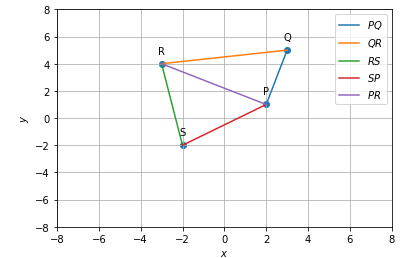
\includegraphics[width=\columnwidth]{2/solution/2/9/2/QUAD.PNG}
    \caption{Quadrilateral PQRS}
    \label{2/9/2fig:Quad PQRS}
\end{figure}


